\chapter{Ergebnisse}
\label{chap:results}

Die in Abschnitt \ref{sec:measurements} beschriebenen Messungen der Umlaufzeiten (Round-Trip-Times;RTT) verschiedener DNS-Anfragen ergaben die in Abbildung \ref{img:results-times} dargestellten Zeiten. Aus diesen Werten ergeben sich nun folgende Ergebnisse.

\paragraph{Performance Einbußen durch DoT}
Wie schon in Kapitel \ref{chap:implementation} näher ausgeführt, war ein Performanceverlust durch den Einsatz von DoT zu erwarten. Dieser schlägt sich speziell in den Minimalzeiten mit ca. 50-100\% Erhöhung nieder. Dies ist auf den notwendigen Verbindungsaufbau zurückzuführen. Diese Werte decken sich grob mit den früheren Messwerten aus der Arbeit von Zhu et al.\cite{Zhu2015} und zeichnen sogar ein etwas besseres Bild. Die durchschnittlichen RTTs der herkömmlichen DNS-Abfragen über UDP betragen dabei 105ms, wobei die über TLS mit 115-128ms um ca. 20\% erhöht sind.

\paragraph{Auswirkung des NAT-Servers}
Vergleicht man nun die Werde der Variante mit und ohne Anonymisierung mittels NAT so erkennt man nur minimale Unterschiede. Ja nach Implementation wurde Unterschiede von 5-11ms beobachtet, was bei einer Gesamtdauer von ca. 120ms 5-9\% ausmacht. Da es zu den alternativen Anonymisierungstechnologien EncDNS und ODNS keine aktuellen Implementierungen gibt, kann dieser Zeitverlust mit keiner Alternative verglichen werden.

\begin{figure}[hb]
    \centering
    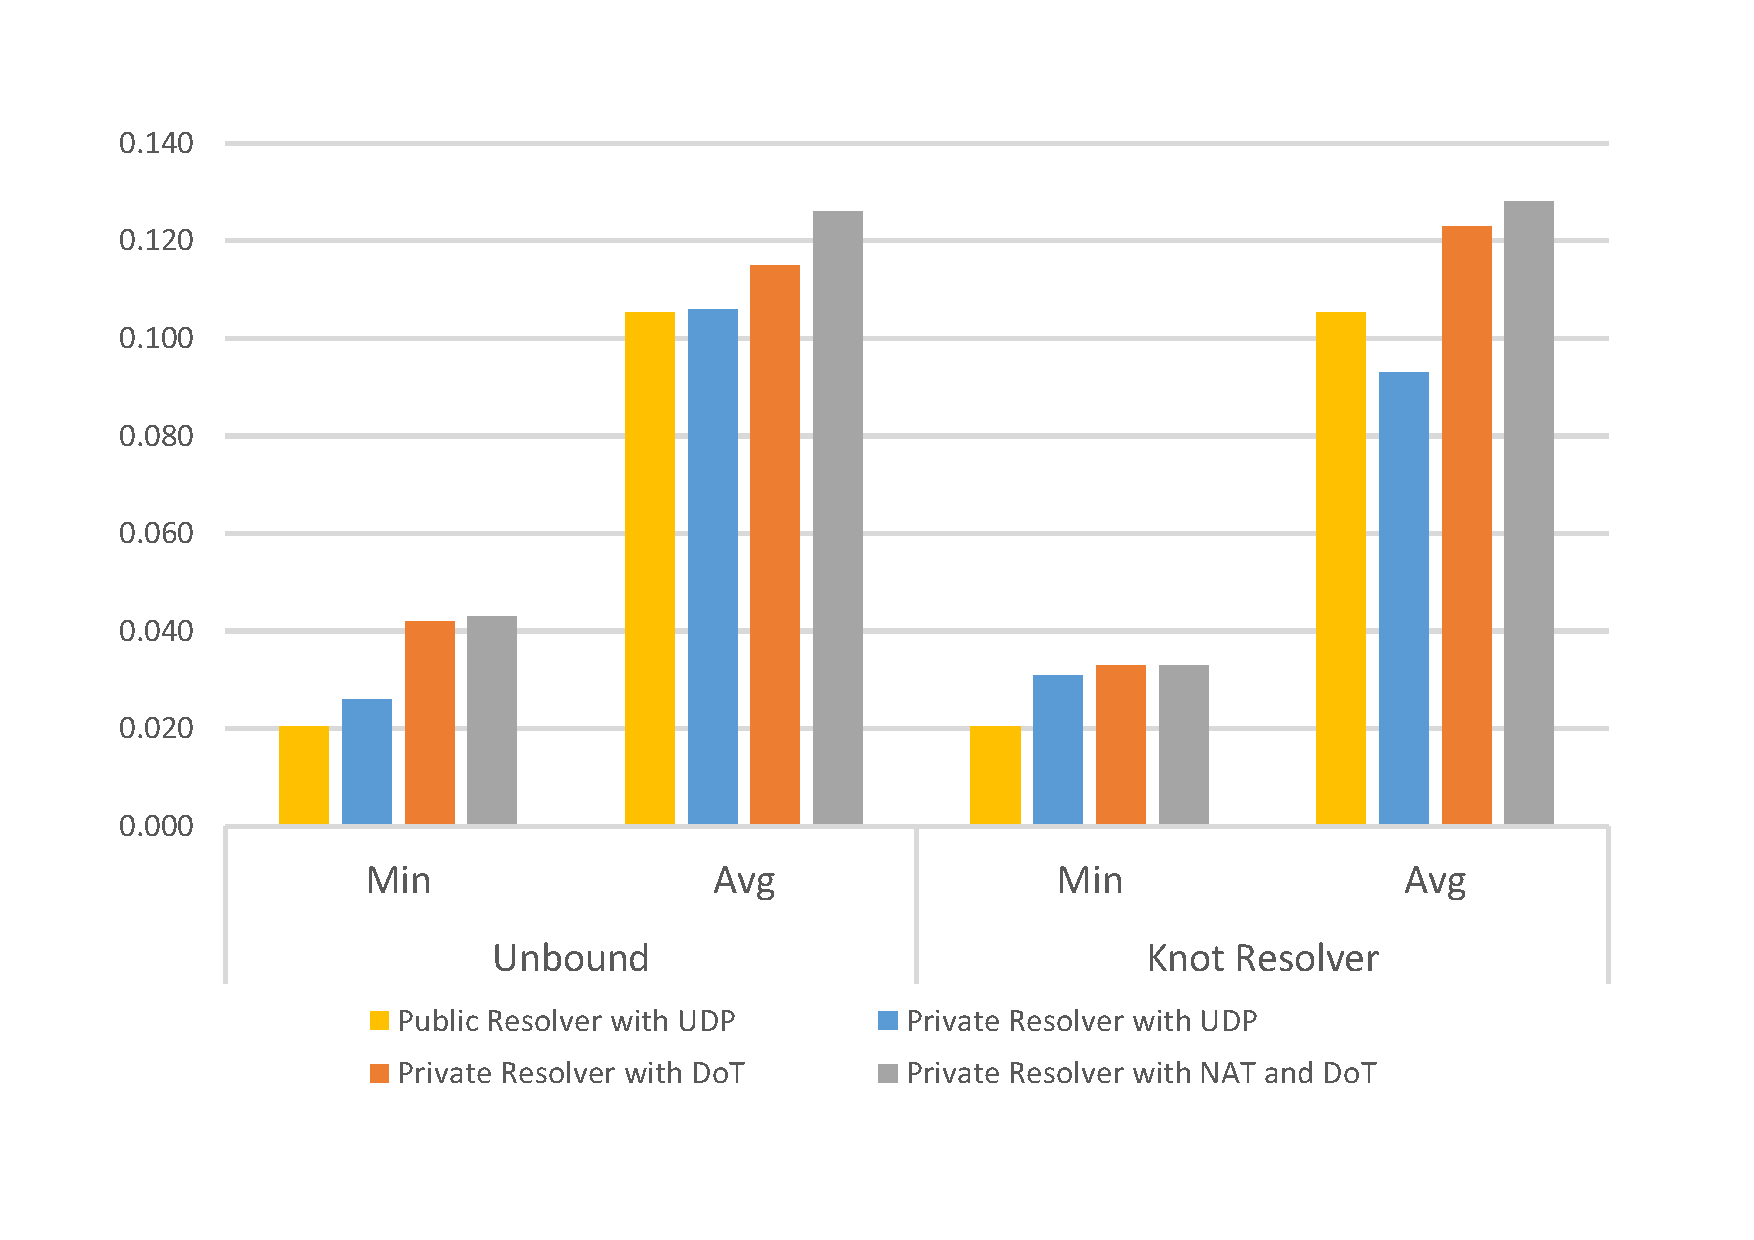
\includegraphics[width=0.6\textwidth]{Results_ResponseTimes}
    \caption{Balkendiagramm der Umlaufzeiten von DNS-Anfragen bei verschiedenen varianten des dargelegten Aufbaus. Die Werte sind in Sekunden angegeben. Die Minimal- (min.) und Durchschnittswerte (avg.) ergeben sich aus Messungen mit dem Programm ``DNS Benchmark'' von Steve Gibson}
    \label{img:results-times}
\end{figure}